\documentclass[11pt,a4paper]{article}
\usepackage[margin=25mm]{geometry}
\usepackage[T1]{fontenc}
\usepackage[utf8]{inputenc}
\usepackage{lmodern}
\usepackage{amsmath,amssymb,amsthm}
\usepackage{booktabs,graphicx}
\usepackage{microtype}
\usepackage{xurl}
\usepackage[hidelinks]{hyperref}
\urlstyle{same}
\hypersetup{
  pdftitle={Quantitative robust estimation for Gaussian inverse problems},
  pdfsubject={Research draft: uniform additive robust-risk bound and exact isotropic-jitter boundary}
}
\providecommand{\tightlist}{%
  \setlength{\itemsep}{0pt}\setlength{\parskip}{0pt}}
\setcounter{secnumdepth}{2}
\setlength{\emergencystretch}{3em}
\allowdisplaybreaks[2]
\title{Quantitative robust estimation for Gaussian inverse
problems\\[0.5em]{\large A proof of the spectral conjecture and an exact
boundary for isotropic input jittering}}
\author{Anonymous}
\date{18 October 2026}
\begin{document}
\maketitle

\hypertarget{abstract}{%
\section*{Abstract}\label{abstract}}
\addcontentsline{toc}{section}{Abstract}

Krainovic, Soltanolkotabi and Heckel proposed a spectral estimator for
Gaussian linear inverse problems by interchanging expectation and
minimisation in a scalar trust-region dual. We prove its asymptotic
optimality among all linear estimators, with a finite-dimensional
additive robust-risk bound uniform over every forward operator, aspect
ratio, measurement-noise level and positive adversarial radius.
Normalised by signal energy, the regret is at most

\[
\min\left\{1,\frac{2^{7/4}}{3^{3/4}}d^{-1/4}+\sqrt2\,d^{-1/2}\right\}.
\]

The proof combines exact symmetry reduction, gain clipping and a
Gaussian quadratic-process estimate controlling the singular dual
boundary. An invariant version of the dual-gap estimate allows arbitrary
Gaussian residual covariance. When the minimising dual parameter is positive, an explicit
anisotropic training-noise covariance implements the spectral rule
through ordinary population least squares. Under positive noise and
active estimation, finite isotropic jittering implements that rule
precisely when the positive singular spectrum is flat. Fixed unequal
spectral bands yield a strictly positive limiting true-risk gap. A
two-band example has a short analytic certificate giving a limiting gap
greater than \(0.141382\) at unit signal energy, and a true
finite-dimensional gap greater than \(0.007292\) at \(d=20000\). The
source's estimator formula and qualitative spectral comparison are
credited explicitly; the contributions here are quantitative proofs,
precise conditions and exact certificates.

\hypertarget{problem-source-and-scope}{%
\section{Problem, source and scope}\label{problem-source-and-scope}}

Let \(d,m,n\) be positive integers with \(n\ge d\). Let
\(U\in\mathbb R^{n\times d}\) satisfy \(U^TU=I_d\), and let
\(A\in\mathbb R^{m\times n}\) be arbitrary. Consider

\[
x=Uc,\qquad c\sim\mathcal N(0,aI_d),\qquad
z\sim\mathcal N(0,bI_m),\qquad
a=\frac E d>0,\qquad b=\frac{\sigma_z^2}{m}\ge0,
\tag{1}
\]

where \(c\) and \(z\) are independent and
\(E=\sigma_c^2=\mathbb E\|x\|^2\) is the signal energy. For
\(\varepsilon>0\) and \(H\in\mathbb R^{n\times m}\), define

\[
\mathcal R_\varepsilon(H)=
\mathbb E\left[\max_{\|e\|\le\varepsilon}
\|H(Ax+z+e)-x\|^2\right].
\tag{2}
\]

All vector norms are Euclidean. The adversarial maximum is inside the
expectation: every realised sample has a separate perturbation budget.

Krainovic, Soltanolkotabi and Heckel {[}1, Conjecture 3.3{]} proposed an
asymptotically optimal spectral estimator for (2), obtained by taking
expectation before minimising a scalar trust-region dual. Their paper
already supplies the spectral formula, dual representation and proposed
interchange. The theorem below gives a uniform quantitative
justification.

The conclusion compares linear estimators only. It requires no
condition-number bound, limiting spectral distribution, fixed aspect
ratio, positive measurement-noise assumption or positive lower bound on
the nonzero singular values. The radius and noise level may depend on
dimension. The conclusion is convergence of additive risk divided by
signal energy, not a risk-ratio assertion or convergence of estimator
matrices.

\hypertarget{relation-to-other-robust-estimation-problems}{%
\subsection{Relation to other robust-estimation
problems}\label{relation-to-other-robust-estimation-problems}}

Zhang, Lee, Hassani and Matni {[}2{]} study per-realisation norm-bounded
attacks in robust state estimation and linear inverse problems. Their
inner attack is also a trust-region problem. Their Section 3.1 bounds
the difference between adversarial and standard risks for a fixed
estimator. The estimate proved here instead bounds the gap between an
expected samplewise dual minimum and the minimum of its expectation, and
then uses that estimate to justify a particular spectral estimator. The
distinction concerns the quantity controlled, not the existence of a
scalar dual.

Zhang, Blanchet, Marzouk, Nguyen and Wang {[}3{]} study Bayesian inverse
estimation when an adversary changes a distribution within a Wasserstein
neighbourhood of a nominal model. They establish strong duality and
analyse a Gaussian least-favourable model and a Nash equilibrium. A
Wasserstein transport budget constrains distributional transport cost,
whereas (2) gives every realised measurement its own norm bound. Their
minimax theorem does not itself establish the expectation--infimum
estimate required here. Lotidis, Bambos, Blanchet and Li {[}4{]} also
use Wasserstein model uncertainty, with martingale constraints for
dynamical estimation.

Input jittering in this paper is a population linear-estimation
construction. Iteration-wise noise injection in nonlinear
reconstruction, such as Guan and Davenport {[}5{]}, is a different
procedure. No finite-sample neural-network optimisation guarantee
follows from the results below.

\hypertarget{spectral-estimator-and-main-theorem}{%
\section{Spectral estimator and main
theorem}\label{spectral-estimator-and-main-theorem}}

Choose a singular-value decomposition

\[
AU=WDV^T,
\]

where \(W\in\mathbb R^{m\times m}\) and \(V\in\mathbb R^{d\times d}\)
are orthogonal, and the rectangular diagonal matrix \(D\) has positive
entries \(s_1,\ldots,s_r\), with \(r=\operatorname{rank}(AU)\). Pad the
list by \(s_i=0\) for \(r<i\le d\), and put \(t=b/a\).

For \(\lambda\ge0\), set

\[
C_i(\lambda)=1+\lambda(s_i^2+t),\qquad
h_i(\lambda)=
\begin{cases}
\displaystyle
\frac{2\lambda s_i}
{C_i(\lambda)+\sqrt{C_i(\lambda)^2-4\lambda s_i^2}},
&s_i>0,\\[8pt]
0,&s_i=0.
\end{cases}
\tag{3}
\]

In particular \(h_i(0)=0\). The discriminant is nonnegative since

\[
C_i(\lambda)^2-4\lambda s_i^2
=[1-\lambda(s_i^2+t)]^2+4\lambda t.
\]

The rationalised root avoids subtraction of nearly equal numbers. Define

\[
\Phi(\lambda)=\lambda\varepsilon^2+
\frac a2\sum_{i=1}^d
\left[
1-\lambda(s_i^2+t)
+\sqrt{[1+\lambda(s_i^2+t)]^2-4\lambda s_i^2}
\right].
\tag{4}
\]

Choose any minimiser \(\lambda_*\ge0\) of \(\Phi\). Let
\(K_*\in\mathbb R^{d\times m}\) have diagonal entries
\(h_i(\lambda_*)\), \(i\le r\), and every other entry zero. Set

\[
H_*=UVK_*W^T.
\tag{5}
\]

\textbf{Theorem 1 (uniform asymptotic optimality).} The objective
\(\Phi\) is continuous and convex and has a minimiser in
\([0,E/\varepsilon^2]\). Define

\[
\eta_d=\frac{2^{7/4}}{3^{3/4}}d^{-1/4}+\sqrt2\,d^{-1/2}.
\tag{6}
\]

Then

\[
0\le\mathcal R_\varepsilon(H_*)-\inf_H\mathcal R_\varepsilon(H)
\le E\min\{1,\eta_d\}.
\tag{7}
\]

Writing \(V=\min_{\lambda\ge0}\Phi(\lambda)\), the untruncated value
comparison is

\[
V-E\eta_d
\le\inf_H\mathcal R_\varepsilon(H)
\le\mathcal R_\varepsilon(H_*)\le V.
\tag{8}
\]

Since \(V\le E\) and all risks are nonnegative, \(E\eta_d\) in the lower
bound can also be replaced by \(E\min\{1,\eta_d\}\). Thus, for arbitrary
sequences of operators, dimensions, noise levels and positive radii, the
regret divided by \(E\) tends to zero as \(d\to\infty\).

The simpler leading constant \(2^{5/4}\) follows from the same proof. We
give both calculations below. Neither the rate exponent nor the leading
constant is asserted to be optimal.

\hypertarget{exact-symmetry-reduction-and-clipping}{%
\section{Exact symmetry reduction and
clipping}\label{exact-symmetry-reduction-and-clipping}}

\hypertarget{existence-and-diagonal-reduction}{%
\subsection{Existence and diagonal
reduction}\label{existence-and-diagonal-reduction}}

Projecting the output of \(H\) onto \(\operatorname{range}(U)\) cannot
increase the error for any \(x,z,e\). It is therefore enough to take
\(H=UL\). Orthogonal changes of signal and measurement coordinates by
\(V\) and \(W\) reduce the problem to estimating
\(c\sim\mathcal N(0,aI_d)\) from \(Dc+z\) by a matrix
\(K\in\mathbb R^{d\times m}\), with the same isotropic noise and
adversarial ball.

The risk is convex in \(K\): each fixed-sample, fixed-perturbation loss
is a convex quadratic, and a maximum followed by an expectation
preserves convexity. Let \(T\) and \(S\) be diagonal sign matrices in
signal and measurement space satisfying \(SD=DT\). Use the same sign on
the two coordinates corresponding to each positive singular value and
independent signs on every remaining coordinate. Isotropy and invariance
of the ball imply

\[
\mathcal R_\varepsilon(TKS)=\mathcal R_\varepsilon(K).
\]

Averaging \(K\) over this finite group removes every entry except
\(K_{ii}\) for \(i\le r\). Convexity shows that the averaged diagonal
estimator has no larger risk.

The risk is continuous in each fixed finite-dimensional matrix space. On
a bounded set of matrices, dominated convergence applies with a constant
multiple of \(\|c\|^2+\|z\|^2+\varepsilon^2\) as a bound. Choose a
deterministic \(e_0\) such that \(\|e_0\|=\varepsilon\) and
\(\|Ke_0\|=\varepsilon\|K\|_{\mathrm{op}}\). Averaging the losses at
\(e_0\) and \(-e_0\) gives

\[
\mathcal R_\varepsilon(K)\ge
\mathbb E\|K(Dc+z)-c\|^2
+\varepsilon^2\|K\|_{\mathrm{op}}^2.
\tag{9}
\]

Thus sublevel sets are compact and a minimiser exists. A diagonal
minimiser may be chosen. The zero estimator has risk \(ad=E\).

For a diagonal estimator with gains \(h_i\), the residual coordinates
are independent centred Gaussians with variances

\[
q_i=a(1-s_i h_i)^2+b h_i^2\quad(i\le r),\qquad
q_i=a\quad(i>r).
\tag{10}
\]

Pad \(h_i=0\) for \(i>r\). This padding introduces no effective
adversarial directions, including when \(m<d\).

\hypertarget{clipping-and-residual-dispersion}{%
\subsection{Clipping and residual
dispersion}\label{clipping-and-residual-dispersion}}

For \(s_i>0\), clip the gain to

\[
0\le h_i\le h_i^0,\qquad
h_i^0=\frac{a s_i}{a s_i^2+b}=\frac{s_i}{s_i^2+t}.
\tag{11}
\]

Clipping decreases both \(|h_i|\) and \(q_i\). The variance is a convex
quadratic minimised at \(h_i^0\), its value at zero is \(a\), and a
negative gain has variance at least \(a\).

To justify risk monotonicity, temporarily regard the gains \(h\) and
variances \(q\) as independent inputs. For fixed \(h\), the function

\[
v\longmapsto\max_{\|e\|\le\varepsilon}\|v+\operatorname{diag}(h)e\|^2
\]

is convex. Increasing the Gaussian variances coordinatewise is
equivalent to adding an independent centred Gaussian vector. Conditional
Jensen's inequality shows that this cannot decrease expected loss. For
fixed \(v\), reducing \(|h_i|\) coordinatewise shrinks the perturbation
ellipsoid, so cannot increase its maximum loss. Applying the two facts
successively proves that clipping cannot increase risk.

For a clipped diagonal robust minimiser, set

\[
B=\max_i|h_i|,\qquad Q_0=\sum_iq_i,\qquad
C=\left(2\sum_iq_i^2\right)^{1/2}.
\]

Then \(0\le q_i\le a\) and (9) gives

\[
Q_0+\varepsilon^2B^2\le E,\qquad
\sum_iq_i^2\le aQ_0,\qquad
C\le\sqrt{\frac2d}\,E.
\tag{12}
\]

This is the uniform residual-dispersion bound. It does not depend on the
singular values or on the choice of the robust minimiser.

\hypertarget{scalar-dual-and-uniform-expectationinfimum-estimate}{%
\section{Scalar dual and uniform expectation--infimum
estimate}\label{scalar-dual-and-uniform-expectationinfimum-estimate}}

\hypertarget{trust-region-identity-including-singular-boundaries}{%
\subsection{Trust-region identity, including singular
boundaries}\label{trust-region-identity-including-singular-boundaries}}

For \(v,h\in\mathbb R^d\) and \(B=\max_i|h_i|\), the trust-region
identity is

\[
\max_{\|e\|\le\varepsilon}\|v+\operatorname{diag}(h)e\|^2
=\inf_{\lambda>B^2}
\left[
\lambda\varepsilon^2+
\sum_i v_i^2\frac{\lambda}{\lambda-h_i^2}
\right].
\tag{13}
\]

Square completion gives the upper bound for every \(\lambda>B^2\). The
stationary attack is

\[
e_i(\lambda)=\frac{h_i v_i}{\lambda-h_i^2}.
\]

Its norm is continuous and nonincreasing in \(\lambda\) and tends to
zero at infinity. If its norm reaches \(\varepsilon\) at a strictly
feasible \(\lambda\), substitution attains equality. Otherwise let
\(\lambda\downarrow B^2\). When \(B>0\), finiteness of the limiting norm
forces \(h_i v_i=0\) in the top eigenspace. Any missing attack norm can
then be added in that eigenspace, giving the limiting value. This is the
usual hard case. If \(B=0\), both sides of (13) equal \(\|v\|^2\). The
strict-domain infimum therefore handles all singular boundaries without
an inverse of a singular matrix.

For independent standard Gaussian \(g_i\), set \(v_i=\sqrt{q_i}g_i\) and
define

\[
\begin{aligned}
R(h,q)&=
\mathbb E\inf_{\lambda>B^2}
\left[\lambda\varepsilon^2+
\sum_iq_i g_i^2\frac{\lambda}{\lambda-h_i^2}\right],\\
S(h,q)&=
\inf_{\lambda>B^2}
\left[\lambda\varepsilon^2+
\sum_iq_i\frac{\lambda}{\lambda-h_i^2}\right].
\end{aligned}
\tag{14}
\]

Choosing any fixed deterministic dual parameter before expectation shows
\(R(h,q)\le S(h,q)\).

\textbf{Lemma 2 (uniform dual gap).} For arbitrary \(q_i\ge0\),
\(h_i\in\mathbb R\), \(B=\max_i|h_i|\) and \(C=(2\sum_iq_i^2)^{1/2}\),
every \(\delta>0\) satisfies

\[
0\le S(h,q)-R(h,q)
\le\varepsilon^2\delta+C\left(1+\frac{B^2}{\delta}\right).
\tag{15}
\]

\textbf{Proof.} Write

\[
F_g(\lambda)=\lambda\varepsilon^2+
\sum_iq_i g_i^2\frac{\lambda}{\lambda-h_i^2},
\]

and let \(R_\delta,S_\delta\) be obtained by restricting the
corresponding infima to \(\lambda\ge B^2+\delta\). Each rational summand
is decreasing in \(\lambda\). Replacing \(\lambda\) by
\(\max\{\lambda,B^2+\delta\}\) therefore increases \(F_g\) by at most
\(\varepsilon^2\delta\). Hence

\[
R\le R_\delta\le R+\varepsilon^2\delta,\qquad S\le S_\delta.
\tag{16}
\]

The centred process

\[
X(\lambda)=\sum_iq_i(g_i^2-1)\frac{\lambda}{\lambda-h_i^2}
\]

converges at infinity to \(X(\infty)=\sum_iq_i(g_i^2-1)\), with
\(\mathbb E|X(\infty)|\le C\). Independence and differentiation give

\[
\begin{aligned}
X'(\lambda)&=-\sum_iq_i(g_i^2-1)
\frac{h_i^2}{(\lambda-h_i^2)^2},\\
\mathbb E|X'(\lambda)|
&\le
\left[2\sum_iq_i^2\frac{h_i^4}{(\lambda-h_i^2)^4}\right]^{1/2}
\le\frac{CB^2}{(\lambda-B^2)^2}.
\end{aligned}
\]

The fundamental theorem of calculus and Tonelli's theorem imply

\[
\begin{aligned}
\mathbb E\sup_{\lambda\ge B^2+\delta}|X(\lambda)|
&\le\mathbb E|X(\infty)|
+\int_{B^2+\delta}^{\infty}\mathbb E|X'(u)|\,du\\
&\le C\left(1+\frac{B^2}{\delta}\right).
\end{aligned}
\tag{17}
\]

Since \(\inf(F+X)\ge\inf F-\sup|X|\), one has
\(S_\delta-R_\delta\le\mathbb E\sup|X|\). Combining this with (16)
proves (15). All terms are finite because the cutoff is positive.
\(\square\)

The lemma does not require any relationship between \(q\) and \(h\). Its
argument also works for independent nonnegative unit-mean multipliers
other than \(g_i^2\), with \(C^2\) replaced by the sum of their weighted
variances. Nonnegativity is needed for the cutoff step. The exact
symmetry reduction above still relies on Gaussian rotational invariance.

\hypertarget{surrogate-minimisation-and-completion-of-the-main-proof}{%
\section{Surrogate minimisation and completion of the main
proof}\label{surrogate-minimisation-and-completion-of-the-main-proof}}

\hypertarget{one-coordinate-at-fixed-dual-parameter}{%
\subsection{One coordinate at fixed dual
parameter}\label{one-coordinate-at-fixed-dual-parameter}}

For \(s_i>0\) and \(\lambda>0\), minimise, or take the boundary infimum
of,

\[
\frac{\lambda[a(1-s_i h)^2+b h^2]}{\lambda-h^2},
\qquad |h|<\sqrt\lambda.
\tag{18}
\]

The stationary equation is

\[
s_i h^2-[1+\lambda(s_i^2+t)]h+\lambda s_i=0.
\tag{19}
\]

The smaller root is (3). It belongs to

\[
0\le h_i(\lambda)\le
\min\left\{\sqrt\lambda,\frac{s_i}{s_i^2+t}\right\},
\]

and the coordinate infimum is

\[
\frac a2\left[
1-\lambda(s_i^2+t)
+\sqrt{[1+\lambda(s_i^2+t)]^2-4\lambda s_i^2}
\right].
\tag{20}
\]

For \(b>0\), the minimum is attained in the strict domain. For \(b=0\),
(20) reduces to \(a(1-\lambda s_i^2)_+\) and

\[
h_i(\lambda)=\min\{\lambda s_i,1/s_i\}.
\tag{21}
\]

At \(\lambda s_i^2=1\), the boundary \(h_i^2=\lambda\) has zero residual
variance; it is handled by the limiting dual. For \(s_i=0\), the best
gain is zero and its contribution is \(a\).

Consequently

\[
\inf_h S(h,q(h))=\inf_{\lambda\ge0}\Phi(\lambda).
\tag{22}
\]

These are infima over the same feasible pairs \((h,\lambda)\), not a
minimax interchange. The stated boundary conventions extend the identity
to zero noise and \(\lambda=0\).

Every summand of \(\Phi\) is convex. For \(t>0\) this follows by
differentiating its square root and using
\((s_i^2+t)^2-(t-s_i^2)^2=4s_i^2t\ge0\). For \(t=0\), it is a
positive-part affine function. Since \(\Phi(0)=E\) and each coordinate
contribution is nonnegative, \(\Phi\) is continuous and coercive for
\(\varepsilon>0\) and has a minimiser in \([0,E/\varepsilon^2]\). The
gains at any minimising \(\lambda_*\) attain the minimum surrogate,
including \(\lambda_*=0\) and the noiseless boundary cases.

The translation to {[}1{]} is \(s_i=\lambda_i\), \(h_i=\sigma_i\), and
\(t=(d/m)\sigma_z^2/\sigma_c^2\). The scalar objective and gains agree
algebraically with the source conjecture.

\hypertarget{regret-and-the-sharpened-coefficient}{%
\subsection{Regret and the sharpened
coefficient}\label{regret-and-the-sharpened-coefficient}}

Let \(h_{\mathrm{opt}}\) be a clipped diagonal robust minimiser and
\(h_*\) a surrogate minimiser. Then

\[
\begin{aligned}
R(h_*)-R(h_{\mathrm{opt}})
&\le S(h_*)-R(h_{\mathrm{opt}})\\
&\le S(h_{\mathrm{opt}})-R(h_{\mathrm{opt}}).
\end{aligned}
\tag{23}
\]

Apply Lemma 2 to \(h_{\mathrm{opt}}\). The direct inequalities
\(C\le\sqrt2E/\sqrt d\) and \(B^2\le E/\varepsilon^2\), together with
\(\delta=2^{1/4}E/(\varepsilon^2d^{1/4})\), give

\[
R(h_*)-R(h_{\mathrm{opt}})
\le E\left(2^{5/4}d^{-1/4}+\sqrt2d^{-1/2}\right).
\tag{24}
\]

For the improved coefficient, retain the joint constraint in (12):

\[
\begin{aligned}
CB^2
&\le
\frac{\sqrt{2aQ_0}(E-Q_0)}{\varepsilon^2}\\
&\le
\frac{2\sqrt2}{3\sqrt3}\,
\frac{E^2}{\varepsilon^2\sqrt d}.
\end{aligned}
\tag{25}
\]

The last inequality follows from

\[
\max_{0\le Q_0\le E}(E-Q_0)\sqrt{Q_0}
=\frac{2E^{3/2}}{3\sqrt3},
\]

attained at \(Q_0=E/3\), and \(a=E/d\). Optimising the cutoff terms
gives

\[
\inf_{\delta>0}\left(\varepsilon^2\delta+\frac{CB^2}{\delta}\right)
=2\varepsilon\sqrt{CB^2}
\le\frac{2^{7/4}}{3^{3/4}}E d^{-1/4}.
\tag{26}
\]

The equality is an infimum with \(\delta\downarrow0\) if \(CB^2=0\).
Adding \(C\le\sqrt2E d^{-1/2}\) proves the untruncated error bound
\(E\eta_d\).

For the value comparison, write \(V=\min\Phi\). The same calculation
yields

\[
V\le S(h_{\mathrm{opt}})
\le R(h_{\mathrm{opt}})+E\eta_d.
\]

Together with \(R(h_*)\le S(h_*)=V\), this proves (8) first, with the
untruncated error. Since \(V\le E\) and \(R(h_{\mathrm{opt}})\ge0\),
also \(V-R(h_{\mathrm{opt}})\le E\). The lower value bound can therefore
use \(E\min\{1,\eta_d\}\). Finally \(R(h_*)\le V\le E\) and
nonnegativity truncate the regret in the same way. This proves Theorem
1. \(\square\)

The estimate was applied only to an arbitrary clipped robust optimiser,
with constants independent of that optimiser. No unproved uniform
convergence over estimators is assumed.

\hypertarget{invariant-extension-to-correlated-gaussian-residuals}{%
\section{Invariant extension to correlated Gaussian
residuals}\label{invariant-extension-to-correlated-gaussian-residuals}}

\textbf{Proposition 3 (arbitrary Gaussian covariance).} Let
\(v\sim\mathcal N(0,Q)\) in \(\mathbb R^k\), with any
positive-semidefinite covariance \(Q\), and let
\(H\in\mathbb R^{k\times m}\) be arbitrary. Set
\(B=\|H\|_{\mathrm{op}}\) and

\[
\begin{aligned}
R&=\mathbb E\max_{\|e\|\le\varepsilon}\|v+He\|^2,\\
S&=\inf_{\lambda>B^2}
\left[
\lambda\varepsilon^2+
\operatorname{tr}\!\left(Q(I-HH^T/\lambda)^{-1}\right)
\right].
\end{aligned}
\]

For every \(\delta>0\),

\[
0\le S-R\le\varepsilon^2\delta+
\sqrt2\|Q\|_F\left(1+\frac{B^2}{\delta}\right).
\tag{27}
\]

No commutation between \(Q\) and \(HH^T\) is assumed.

\textbf{Proof.} The trust-region dual and cutoff argument are unchanged.
Put

\[
M_\lambda=(I-HH^T/\lambda)^{-1},\qquad
X(\lambda)=v^TM_\lambda v-\operatorname{tr}(QM_\lambda).
\]

For symmetric \(M\), the Gaussian quadratic-form identity gives
\(\operatorname{Var}(v^TMv)=2\operatorname{tr}(QMQM)\). Moreover,

\[
\operatorname{tr}(QMQM)\le\|M\|_{\mathrm{op}}^2\operatorname{tr}(Q^2).
\tag{28}
\]

Indeed, diagonalising \(Q\) with eigenvalues \(q_i\ge0\) gives

\[
\begin{aligned}
\operatorname{tr}(QMQM)
&=\sum_{i,j}q_iq_jM_{ij}^2\\
&\le\frac12\sum_{i,j}(q_i^2+q_j^2)M_{ij}^2\\
&=\sum_iq_i^2(M^2)_{ii}
\le\|M\|_{\mathrm{op}}^2\sum_iq_i^2.
\end{aligned}
\]

At infinity, \(X(\infty)=\|v\|^2-\operatorname{tr}Q\), so
\(\mathbb E|X(\infty)|\le\sqrt2\|Q\|_F\). Also

\[
M'_\lambda=-HH^T(\lambda I-HH^T)^{-2},\qquad
\|M'_\lambda\|_{\mathrm{op}}
\le\frac{B^2}{(\lambda-B^2)^2}.
\]

Using (28), the same integral argument as (17) proves (27). \(\square\)

For \(Q\ne0\), define

\[
d_{\mathrm{eff}}=\frac{(\operatorname{tr}Q)^2}{\operatorname{tr}(Q^2)}.
\]

Then \(\|Q\|_F=\operatorname{tr}Q/\sqrt{d_{\mathrm{eff}}}\). The
covariance bound reflects dispersion of variance; adding zero-variance
coordinates does not improve this scale. The main inverse-problem
theorem uses clipping to obtain the required dispersion uniformly over
its unknown robust optimiser.

\hypertarget{constructive-anisotropic-input-jittering}{%
\section{Constructive anisotropic input
jittering}\label{constructive-anisotropic-input-jittering}}

Assume \(\lambda_*>0\). In the measurement singular-vector basis \(W\),
choose

\[
w_i=\frac{a s_i}{h_i(\lambda_*)}-(a s_i^2+b)
=\frac{a[1-s_i h_i(\lambda_*)]}{\lambda_*}\ge0,
\qquad i\le r.
\tag{29}
\]

For \(r<i\le m\), set \(w_i=a/\lambda_*>0\). Let \(\xi\) be centred
Gaussian, independent of \((c,z)\), with covariance

\[
\operatorname{Cov}(\xi)=
W\operatorname{diag}(w_1,\ldots,w_m)W^T.
\tag{30}
\]

Consider ordinary population least-squares training,

\[
\mathcal J(H)=\mathbb E\|H(Ax+z+\xi)-x\|^2.
\tag{31}
\]

\textbf{Corollary 4 (exact population implementation).} The unique
linear minimiser of (31) is \(H_*\) and therefore satisfies Theorem 1.

\textbf{Proof.} In singular coordinates the linear minimum
mean-square-error gains are

\[
\frac{a s_i}{a s_i^2+b+w_i},\qquad i\le r,
\]

with every other entry zero. Formula (29) makes them exactly
\(h_i(\lambda_*)\). Dividing (19) by \(\lambda_*h_i\) and multiplying by
\(a\) gives the second expression in (29). Since \(0\le s_i h_i\le1\),
the variances are nonnegative. The input covariance is positive on
informative directions because \(a s_i^2>0\), and on all remaining
measurement directions because the chosen \(w_i>0\). Hence the
least-squares minimiser is unique. \(\square\)

The covariance is directly computable. Anisotropic Gaussian noise and
its Wiener-filter algebra are not claimed to be new concepts; the result
pairs this particular covariance with the proved robust-risk
approximation.

If \(\lambda_*=0\), prescribe \(H_*=0\) directly. A finite jitter
covariance cannot produce zero gains on every informative direction, so
that endpoint is excluded from Corollary 4. When \(A=0\), the zero
estimator is already available. When \(b=0\) and \(h_i=1/s_i\), its
required jitter variance is zero, which is valid.

\hypertarget{exact-isotropic-implementation-and-its-boundary}{%
\section{Exact isotropic implementation and its
boundary}\label{exact-isotropic-implementation-and-its-boundary}}

Write \(\kappa=w/a\) for a common isotropic jitter variance relative to
the signal-coordinate variance. Its gains are

\[
h_i^{\mathrm{iso}}(\kappa)=\frac{s_i}{s_i^2+t+\kappa},
\qquad\kappa\ge0.
\tag{32}
\]

The source already identifies equal singular values as an optimality
case and discusses a typically small gap for unequal singular values
{[}1, Section 3.3{]}. The next results turn that comparison into an
exact classification under positive noise and a strict limiting gap for
the true samplewise robust risk.

\textbf{Proposition 5 (flat-spectrum characterisation).} Suppose
\(t>0\), \(\lambda_*>0\), and \(AU\) has at least one positive singular
value. A finite isotropic jitter variance produces exactly \(H_*\) if
and only if all positive singular values of \(AU\) are equal.

\textbf{Proof.} If the isotropic gains equal the proposed robust gains,
(29) gives

\[
\kappa=
\frac{1-s_i h_i^{\mathrm{iso}}(\kappa)}{\lambda_*}
=\frac{t+\kappa}{\lambda_*(s_i^2+t+\kappa)}
\]

for each \(s_i>0\). Equivalently,

\[
\lambda_*\kappa(s_i^2+t+\kappa)=t+\kappa.
\tag{33}
\]

Since \(t>0\), the ratio \(\kappa\) must be positive; (33) then forces
equality of all positive \(s_i^2\). Conversely, if these singular values
agree, (29) gives the same positive ratio on every informative
direction. Using it isotropically yields the same gains. Zero singular
directions have zero reconstruction gain regardless. \(\square\)

For squared singular value \(u>0\), the required ratio solves

\[
\lambda_*\kappa^2+[\lambda_*(u+t)-1]\kappa-t=0.
\tag{34}
\]

It has one positive root, which decreases strictly with \(u\):

\[
\frac{d\kappa}{du}
=-\frac{\lambda_*\kappa}
{2\lambda_*\kappa+\lambda_*(u+t)-1}<0.
\]

The denominator is the positive square root of the quadratic
discriminant. Thus the prescribed covariance injects more training noise
into less informative directions.

Proposition 5 concerns exact equality of estimators. That alone does not
prove a positive finite-dimensional risk gap. The next theorem supplies
the additional limit argument.

\hypertarget{persistent-asymptotic-gap-for-fixed-unequal-bands}{%
\section{Persistent asymptotic gap for fixed unequal
bands}\label{persistent-asymptotic-gap-for-fixed-unequal-bands}}

Normalise \(E=1\). Fix positive singular values \(s_1,\ldots,s_J\),
positive rational proportions \(p_j\) with \(\sum_jp_j=1\), and a
positive noise ratio \(t\). Assume

\[
0<\varepsilon^2<\sum_jp_js_j^2.
\tag{35}
\]

Let \(d\to\infty\) through common multiples of the proportions'
denominators. Take \(m=n=d\), \(U=I_d\), \(c\sim\mathcal N(0,I_d/d)\)
and \(z\sim\mathcal N(0,tI_d/d)\). Let \(A_d\) be diagonal with \(s_j\)
repeated \(p_jd\) times. The operators are deterministic.

For a bandwise constant gain vector \(h\in\mathbb R^J\), write

\[
q_j(h)=(1-s_jh_j)^2+t h_j^2
\]

and

\[
S(h)=
\inf_{\lambda>\max_j h_j^2}
\left[
\lambda\varepsilon^2+
\sum_jp_jq_j(h)\frac{\lambda}{\lambda-h_j^2}
\right].
\tag{36}
\]

The deterministic primal form is

\[
S(h)=
\max_{\sum_j e_j^2\le\varepsilon^2}
\sum_j\left[\sqrt{p_jq_j(h)}+h_j e_j\right]^2.
\tag{37}
\]

It follows from (13) using deterministic residual coordinates
\(\sqrt{p_jq_j(h)}\). Equivalently, in each equal-gain band the worst
perturbation aligns with the band's residual, so only its norm matters.

Define

\[
\begin{aligned}
V_*=\min_{\lambda\ge0}\bigg\{&
\lambda\varepsilon^2+\frac12\sum_jp_j
\left[
1-\lambda(s_j^2+t)
+\sqrt{[1+\lambda(s_j^2+t)]^2-4\lambda s_j^2}
\right]\bigg\},
\\
V_{\mathrm{iso}}&=\inf_{\kappa\ge0}S(h^{\mathrm{iso}}(\kappa)),
\qquad \Delta=V_{\mathrm{iso}}-V_*.
\end{aligned}
\tag{38}
\]

\textbf{Theorem 6 (strict limiting isotropic gap).} If at least two
positive bands have distinct singular values, then \(\Delta>0\) and

\[
\lim_{d\to\infty}
\left[
\inf_{\kappa\ge0}\mathcal R_{\varepsilon,d}(H_{\mathrm{iso}}(\kappa))
-\inf_H\mathcal R_{\varepsilon,d}(H)
\right]=\Delta>0.
\tag{39}
\]

The anisotropic-jitter estimator has risk converging to \(V_*\). If all
singular values in the fixed list agree, then \(\Delta=0\).

\textbf{Proof.} The scalar objective in (38) has derivative
\(\varepsilon^2-\sum_jp_js_j^2<0\) at zero. It therefore has a positive
minimiser. The minimiser is unique because its second derivative is

\[
\sum_j
\frac{2p_js_j^2t}
{\left([1+\lambda(s_j^2+t)]^2-4\lambda s_j^2\right)^{3/2}}>0.
\tag{40}
\]

At \(\lambda_*>0\), every coordinate minimisation has a unique interior
gain because \(t>0\).

The full surrogate has a unique gain minimiser. A minimising vector
cannot be zero because \(V_*<1=S(0)\). For a nonzero vector, every
\(q_j(h)\) is positive, so its scalar dual objective diverges at the
largest gain pole and at infinity. Its dual optimum is attained in the
strict domain. Equality with \(V_*\) forces that optimum to be
\(\lambda_*\) and forces every coordinate gain to its unique minimiser.
Thus \(h_*\) is the only minimising gain vector.

The isotropic path extends continuously to \(\kappa=\infty\) by
\(h^{\mathrm{iso}}(\infty)=0\). Formula (37) makes \(S\) continuous in
\(h\). Hence the isotropic objective is continuous on the
compactification \([0,\infty]\) and attains its infimum. The endpoint at
infinity has value \(1>V_*\). At finite \(\kappa\), Proposition 5
excludes equality with \(h_*\) whenever two bands differ. Uniqueness of
the global surrogate minimiser yields \(V_{\mathrm{iso}}>V_*\).

For every \(\kappa\), the isotropic gains are clipped and the
dimension-\(d\) residual coordinate variances are at most \(1/d\). Their
operator norms obey the fixed bound

\[
\overline B=\max_j\frac{s_j}{s_j^2+t}<\infty.
\]

Lemma 2 therefore gives, uniformly over \(\kappa\ge0\),

\[
0\le S(h^{\mathrm{iso}}(\kappa))
-\mathcal R_{\varepsilon,d}(H_{\mathrm{iso}}(\kappa))
\le\varepsilon^2\delta+
\sqrt{2/d}\left(1+\frac{\overline B^2}{\delta}\right).
\tag{41}
\]

Taking \(\delta=d^{-1/4}\) makes the right side tend to zero. The best
true isotropic risk tends to \(V_{\mathrm{iso}}\). For these repeated
bands, the scalar objective of Theorem 1 is exactly (38), so (8) shows
that the global optimal linear risk and the selected spectral risk both
tend to \(V_*\). Their difference gives (39). For a flat spectrum, one
isotropic variance implements \(h_*\), proving the converse. \(\square\)

At general fixed signal energy \(E\), the activity condition becomes
\(\varepsilon^2<E\sum_jp_js_j^2\). Risks are \(E\) times their
normalised counterparts with radius squared \(\varepsilon^2/E\). The
result is an additive risk difference.

\hypertarget{an-analytic-two-band-separation-certificate}{%
\section{An analytic two-band separation
certificate}\label{an-analytic-two-band-separation-certificate}}

Take

\[
(s_1,s_2)=\left(\frac25,1\right),\qquad
(p_1,p_2)=\left(\frac15,\frac45\right),\qquad
t=\frac1{1000},\qquad
\varepsilon^2=\frac15,\qquad E=1.
\tag{42}
\]

Condition (35) holds because \(\sum_jp_js_j^2=104/125\). Dimensions may
be \(5,10,15,\ldots\).

For orientation, numerical scalar optimisation gives
\(\lambda_*\simeq1.0419687516\), spectral gains
\((0.4162671156,0.9827181294)\), required anisotropic ratios
\((0.7999214491,0.0165857858)\), and \(V_*\simeq0.3889178775\). The best
isotropic ratio is approximately \(0.3793690380\), with
\(V_{\mathrm{iso}}\simeq0.5312794237\) and gap approximately
\(0.1423615462\). The proof below does not rely on these decimals,
numerical optimisation or a grid.

\textbf{Proposition 7 (analytic separation).} For (42),

\[
V_{\mathrm{iso}}\ge\frac{5303}{10000}=0.5303,\qquad
V_*<\frac{388918}{1000000}=0.388918,
\]

and consequently

\[
\Delta>\frac{141382}{1000000}=0.141382.
\tag{43}
\]

\textbf{Proof: lower bound.} Put \(c=\kappa+t>0\). The isotropic gains
and variances satisfy

\[
h_j=\frac{s_j}{s_j^2+c},\qquad
q_j=\frac{c^2+t s_j^2}{(s_j^2+c)^2},
\qquad
\sqrt{q_j}\ge\frac{c}{s_j^2+c}.
\tag{44}
\]

Use the single fixed feasible attack

\[
e=\frac{(4,3)}{5\sqrt5},\qquad
e_1^2+e_2^2=\frac15.
\]

All entries are nonnegative. Substituting into (37), then using (44),
gives

\[
S(h^{\mathrm{iso}}(\kappa))\ge L(c)
:=\frac15\left[
\left(\frac{c+8/25}{c+4/25}\right)^2+
\left(\frac{2c+3/5}{c+1}\right)^2
\right].
\tag{45}
\]

Set \(y=25c\ge0\). Exact algebra gives

\[
L(c)-\frac{5303}{10000}
=\frac{F(y)}{10000(y+4)^2(y+25)^2},
\tag{46}
\]

\noindent\begin{minipage}{\linewidth}
where

\[
F(y)=4697y^4+8426y^3-1004423y^2+1162600y+34170000.
\tag{47}
\]
\end{minipage}

The following identity proves positivity without root approximation:

\[
\begin{aligned}
F(y)={}&(y-9)^2(4697y^2+92972y+288616)\\
&-1173044(y-9)+234708.
\end{aligned}
\tag{48}
\]

For \(0\le y\le9\), all terms on the right are nonnegative and the
constant term is positive. For \(y\ge9\), write \(z=y-9\ge0\). The
quadratic coefficient in parentheses is increasing for \(y\ge0\) and has
value \(1505821\) at \(y=9\). Thus

\[
F(y)\ge1505821z^2-1173044z+234708.
\]

This quadratic has positive leading coefficient and discriminant

\[
1173044^2-4\cdot1505821\cdot234708
=-37680715136<0.
\tag{49}
\]

Therefore \(F(y)>0\) for every \(y\ge0\). Equations (45)--(46) give the
claimed uniform lower bound on \(V_{\mathrm{iso}}\).

\textbf{Proof: upper bound.} Choose the rational feasible dual and gain
tuple

\[
\lambda=\frac{104196875}{10^8},\qquad
h_1=\frac{416267115648}{10^{12}},\qquad
h_2=\frac{982718129443}{10^{12}}.
\tag{50}
\]

Both inequalities \(\lambda>h_j^2\) hold. With
\(q_j=(1-s_jh_j)^2+t h_j^2\), the gap between \(0.388918\) and its
feasible dual value is exactly

\[
\begin{aligned}
&\frac{388918}{10^6}
-\left[\lambda\varepsilon^2+
\sum_jp_jq_j\frac{\lambda}{\lambda-h_j^2}\right]\\
&\quad=
\frac{3168557554921612509053869041613787853379731}
{25868592782876951709628705995150319490966201600000}
>0.
\end{aligned}
\tag{51}
\]

Since \(V_*\) is the minimum over all feasible gains and dual
parameters, (51) proves the strict upper bound. Subtracting proves (43).
\(\square\)

\hypertarget{explicit-finite-dimensional-separation}{%
\subsection{Explicit finite-dimensional
separation}\label{explicit-finite-dimensional-separation}}

\textbf{Corollary 8.} For (42) and every positive dimension \(d\)
divisible by five,

\[
\begin{aligned}
&\inf_{\kappa\ge0}\mathcal R_{\varepsilon,d}(H_{\mathrm{iso}}(\kappa))
-\inf_H\mathcal R_{\varepsilon,d}(H)\\
&\qquad>
\frac{141382}{1000000}
-\left(\frac{128}{27d}\right)^{1/4}
-\sqrt{\frac2d}.
\end{aligned}
\tag{52}
\]

At \(d=20000\), and at every larger multiple of five, this true risk
difference is strictly greater than \(0.007292\).

\textbf{Proof.} At each fixed dimension, the isotropic path compactifies
continuously by the zero estimator at \(\kappa=\infty\). The risk is
continuous on that compactification by dominated convergence because
gains and residual second moments are uniformly bounded. A best
estimator on the compactification exists and its risk is at most one.
The finite-\(\kappa\) infimum has the same value, since zero is a limit
of finite-\(\kappa\) estimators.

At a minimising isotropic estimator, all coordinate variances are at
most \(1/d\), and (9) gives \(Q_0+\varepsilon^2B^2\le1\). The sharpened
calculation (25)--(26) therefore bounds its surrogate-minus-true-risk
gap by

\[
\eta_d=\left(\frac{128}{27d}\right)^{1/4}+\sqrt{\frac2d}.
\]

Its surrogate value is at least \(V_{\mathrm{iso}}\), whereas the global
optimal linear true risk is at most \(V_*\). The difference is at least
\(\Delta-\eta_d\), and (43) makes (52) strict. This coercivity bound is
applied at a best isotropic estimator, not asserted uniformly over every
isotropic gain.

The numerical dimension threshold also follows from exact arithmetic:

\[
\left(\frac{12409}{100000}\right)^4-\frac{128}{27\cdot20000}
=
\frac{192972343173947}{2700000000000000000000}>0,
\qquad
\sqrt{\frac2{20000}}=\frac1{100}.
\tag{53}
\]

Hence \(\eta_{20000}<0.13409\) and \(0.141382-0.13409=0.007292\). Since
\(\eta_d\) decreases with \(d\), the same lower bound holds for every
larger allowed dimension. \(\square\)

\begin{figure}[htbp]
\centering
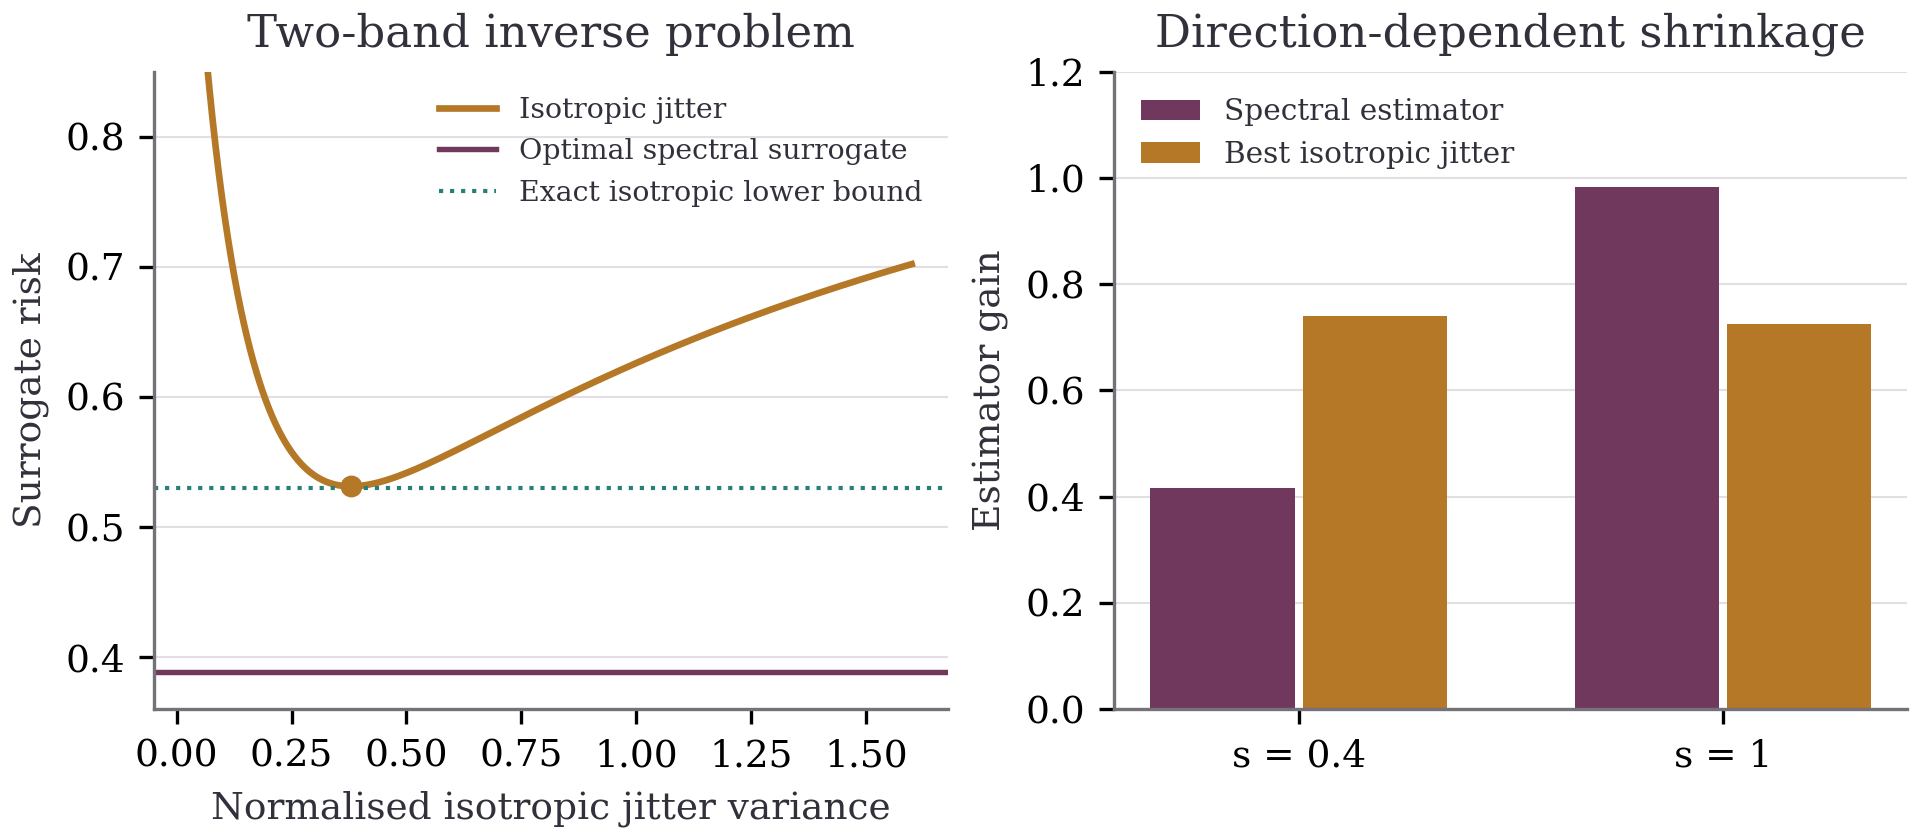
\includegraphics[width=\linewidth]{figures/inverse_jitter_illustration.png}
\caption{Numerical illustration of the two-band problem (42). The curves
show the deterministic surrogate and the exact isotropic lower bound
$0.5303$; the bars compare the numerically minimising gains. The separation
is proved by the rational certificate (44)--(51), independently of these
plots or numerical optimisation.}
\label{fig:inverse}
\end{figure}

\hypertarget{endpoint-checks-reproducibility-and-limitations}{%
\section{Endpoint checks, reproducibility and
limitations}\label{endpoint-checks-reproducibility-and-limitations}}

At \(A=0\), the proposed gains are all zero and both true and surrogate
risks equal \(E\). For \(A=I_n\), \(b=0\) and \(\varepsilon<\sqrt E\),
all \(d\) informative singular values equal one, so

\[
\Phi(\lambda)=\lambda\varepsilon^2+E(1-\lambda)_+.
\]

Its minimum is at \(\lambda=1\) and gives \(H_*=UU^T\), with robust risk
exactly \(\varepsilon^2\). This equals \(I_n\) only in the
full-dimensional case. At \(\varepsilon=0\), the usual linear minimum
mean-square-error estimator is exactly optimal; its informative gains
arise as \(\lambda\to\infty\). The positive-radius coercivity argument
is not needed at that separate endpoint.

The deterministic surrogate need not be the exact finite-dimensional
optimum. In a scalar problem with \(a=s=1\), \(b=0\) and
\(\sqrt{2/\pi}<\varepsilon<1\), the prescribed gain is \(h_*=1\). For
\(0\le h\le1\), however,

\[
R(h)=(1-h)^2+\varepsilon^2h^2
+2\varepsilon\sqrt{2/\pi}\,h(1-h).
\tag{54}
\]

Its left derivative at \(h=1\) is positive, so a slightly smaller gain
reduces true risk. At \(\varepsilon=0.9\), the prescribed risk is
\(0.81\), while the scalar minimum is approximately \(0.7874046283\) at
\(h\simeq0.7541413058\). This confirms the need for an asymptotic risk
statement.

The exact symmetry, clipping and boundary arguments cover rectangular
measurements, rank deficiency and zero measurement noise. In contrast,
the isotropic classification and fixed-band gap use their stated
additional hypotheses: positive noise ratio and positive dual minimiser,
and for the gap theorem, positive fixed band proportions and the
active-estimation condition (35). These conditions must not be dropped
by importing the broader scope of Theorem 1.

The central proof is analytic. The polynomial identities and rational
inequalities in the final certificate are displayed explicitly so that
they can be checked with integer and rational arithmetic. Numerical
optimisation is used only for the illustrative decimal values.
Independent internal agents examined the proof, reproduced exact
arithmetic and checked the statement against the originating source.
These checks are not external peer review or proof-assistant
formalisation.

The recorded prior-art search was last checked on 17 October 2026. It
located the originating conjecture and adjacent work, but no later proof
of the exact general statement in the searched corpus. This is bounded
evidence, not proof of historical priority. The estimator formula,
trust-region dual, isotropic Wiener gains and qualitative spectral
limitation are credited to the source. The paper does not establish
optimality over nonlinear estimators, an optimal convergence exponent or
constant, a matrix-norm convergence rate, or practical neural-network
training guarantees.

\section*{Claim-to-evidence map}
\addcontentsline{toc}{section}{Claim-to-evidence map}

\begin{center}
\small
\begin{tabular}{@{}p{0.24\linewidth}p{0.27\linewidth}p{0.21\linewidth}p{0.20\linewidth}@{}}
\toprule
Claim & Analytic support & Executable support & Not established by the check \\
\midrule
Uniform additive regret bound & Theorem 1, Lemma 2, (23)--(26) & \path{inverse_risk_checks.py} finite cases & the uniform theorem itself \\
Arbitrary-covariance dual gap & Proposition 3 & analytic proof; no packaged executable check & optimality of the constant \\
Anisotropic implementation & Corollary 4 and (29) & related scalar-root and spectral-gain checks only & the covariance identity or finite-sample guarantees \\
Isotropic boundary and persistent gap & Proposition 5 and Theorem 6 & one-positive-band finite checks plus exact two-band certificate & the analytic general theorem or equality outside its hypotheses \\
Explicit two-band separation & Proposition 7 and Corollary 8 & \path{analytic_isotropic_gap.py} exact arithmetic & optimality of the example or dimension threshold \\
\bottomrule
\end{tabular}
\end{center}

\hypertarget{references}{%
\section*{References}\label{references}}
\addcontentsline{toc}{section}{References}

\begin{enumerate}
\def\labelenumi{\arabic{enumi}.}
\item
  Krainovic, A., Soltanolkotabi, M., \& Heckel, R. (2023). Learning
  provably robust estimators for inverse problems via jittering.
  \emph{Advances in Neural Information Processing Systems, 36},
  57276--57305. Primary proceedings text:
  \url{https://proceedings.neurips.cc/paper_files/paper/2023/file/b3411e30afa6caeefa4d6d39a5ea84cd-Paper-Conference.pdf}.
  Preprint: \url{https://arxiv.org/abs/2307.12822}.
\item
  Zhang, T. T. C. K., Lee, B. D., Hassani, H., \& Matni, N. (2023).
  Adversarial tradeoffs in robust state estimation. \emph{2023 American
  Control Conference}, 4083--4089.
  \url{https://doi.org/10.23919/ACC55779.2023.10156358}. Full author
  version consulted: \url{https://arxiv.org/abs/2111.08864v3}.
\item
  Zhang, X., Blanchet, J., Marzouk, Y., Nguyen, V. A., \& Wang, S.
  (2025). Distributionally robust Gaussian process regression and
  Bayesian inverse problems. \emph{The Annals of Applied Probability,
  35}(3), 1489--1530. \url{https://doi.org/10.1214/24-AAP2141}. Full
  author version consulted: \url{https://arxiv.org/html/2205.13111v5}.
\item
  Lotidis, K., Bambos, N., Blanchet, J., \& Li, J. (2023). Wasserstein
  distributionally robust linear-quadratic estimation under martingale
  constraints. \emph{Proceedings of the 26th International Conference on
  Artificial Intelligence and Statistics}, PMLR 206, 8629--8644.
  \url{https://proceedings.mlr.press/v206/lotidis23a.html}.
\item
  Guan, P., \& Davenport, M. A. (2025). SGD jittering: A training strategy
  for robust and accurate model-based architectures. \emph{Proceedings of
  the 42nd International Conference on Machine Learning, Proceedings of
  Machine Learning Research, 267}, 20553--20571.
  \url{https://proceedings.mlr.press/v267/guan25b.html}. Preprint:
  \url{https://arxiv.org/abs/2410.14667}.
\end{enumerate}

\end{document}
